
%\documentclass[10pt,twoside,twocolumn]{article}
\documentclass[12pt,twoside]{article}
\usepackage[bf,small]{caption}
\usepackage[letterpaper,hmargin=1in,vmargin=1in]{geometry}
\usepackage{paralist} % comapctitem, compactdesc, compactenum
\usepackage{titlesec}
\usepackage{titletoc}
\usepackage{times}
\usepackage{hyperref}
\usepackage{algorithmic}
\usepackage{graphicx}
\graphicspath{{./graphics/}}
\usepackage{xspace}
\usepackage{verbatim}
\usepackage{url}
\usepackage{float}
\hyphenation{Sub-Bytes Shift-Rows Mix-Col-umns Add-Round-Key}

\setlength{\parskip}{12pt}
\setlength{\parindent}{0pt}

\newcommand{\hdb}{\emph{hashdb}\xspace}
\newcommand{\bulk}{\emph{bulk\_extractor}\xspace}
\newcommand{\mdd}{\emph{md5deep}\xspace}
\newcommand{\bev}{\emph{Bulk Extractor Viewer}\xspace}

\begin{document}

\begin{center}
\Large Demo: Finding Fragments of Previously Encountered Data \\
\large using \hdb and \bulk
\end{center}

In this demo, we find that a media image contains part of a
previously encountered video file.
This demo uses the following resources:
\begin{compactitem}
\item A media image containing a fragment of a video file.
\item A \hdb block hash database containing block hashes
from the previously encountered video file.
\item The \hdb tool.
\item \bulk compiled with the \hdb scanner.
\end{compactitem}

Here is the workflow:

\begin{figure}[H]
  \center
  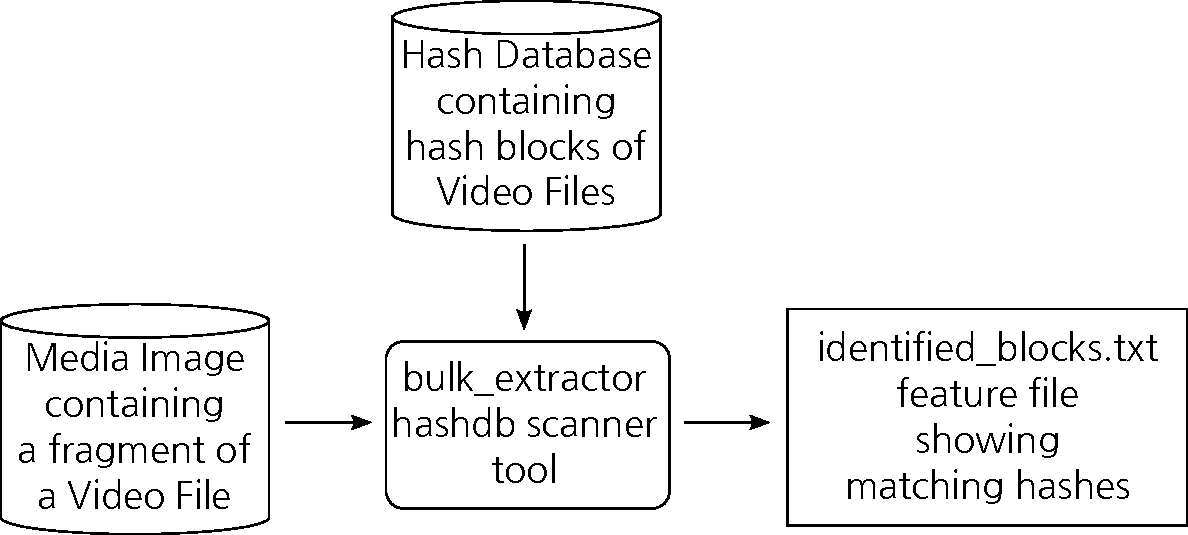
\includegraphics[scale=0.6]{drawings/scan_hashdb}
  \caption*{Scan the media image for parts of a video file.}
  \label{fig:scan_hashdb}
\end{figure}

Setup:
\begin{compactenum}
\item Download and install \hdb from
\url{http://digitalcorpora.org/downloads/hashdb}
as described at
\url{https://github.com/simsong/hashdb/wiki/Installing-hashdb}.
\item Download and install \bulk compiled with \hdb from
\url{http://digitalcorpora.org/downloads/hashdb}
as described at
\url{https://github.com/simsong/hashdb/wiki/Installing-hashdb}.
\item This demo requires hash dtabase \texttt{mock\_video.hdb}
created by demo ``Demo: Creatng a Block Hash Database using \hdb and \mdd''
available at
\url{http://digitalcorpora.org/downloads/hashdb/demo/create\_hdb\_demo.pdf}.
Please follow that demo to create your \texttt{mock\_video.hdb} hash database
and copy it into your current working directory.
\item Download the media file to scan from here:
\url{http://digitalcorpora.org/downloads/hashdb/demo/mock\_video\_redacted\_image}.
This media file contains a fragment of the demo video file,
specifically, a contiguous 64KiB section
near the end of about 10 MiB of video data:
\end{compactenum}
Steps:
\begin{compactenum}
\item Now scan for matching hash values:
Using a command window, go to your working directory and then run \bulk,
specifying the paths to the hash database and the media:
\begin{verbatim}
$ bulk_extractor -e hashdb -o outdir -S hashdb_mode=scan \
  -S hashdb_scan_path_or_socket=mock_video.hdb \
  mock_video_redacted_image
\end{verbatim}
\item View the feature file using an editor or use the \bev tool.
For example to view with Windows Notepad, type:
\begin{verbatim}
$ notepad outdir/identified_blocks.txt
\end{verbatim}
An example hash block match looks like this:
\begin{verbatim}
12452352    3b6b477d391f73f67c1c01e2141dbb17    1
\end{verbatim}
\end{compactenum}

Seeing hash \texttt{3b6b477...} at Forensic path \texttt{12452352}
shows that a hash block match was found, but what file does it match?
We find the file that contains the hash by using a \hdb source lookup:
\begin{figure}[H]
  \center
  
\includegraphics[scale=0.6]{drawings/source_lookup}
  \caption*{Look up the file that has the hash.}
  \label{fig:source_lookup}
\end{figure}

Steps to look up source information about the identified blocks:
\begin{compactenum}
\item Using a command window, go to your working directory and then run
the \hdb tool:
\begin{verbatim}
$ hashdb expand_identified_blocks mock_video.hdb \
  outdir/identified_blocks.txt > outdir/identified_sources.txt
\end{verbatim}

\item Now view file \texttt{outdir/identified\_sources.txt} to see
features containing source information.
This example line:
\begin{verbatim}
12452352    3b6b477d391f73f67c1c01e2141dbb17 \
repository_name=repository_mock_video.xml, \
filename=/home/bdallen/demo/mock_video.mp4, \
file_offset=10485760
\end{verbatim}

states that the block at Forensic path \texttt{12452352}
matches the block \texttt{10485760} bytes into the
\texttt{mock\_video.mp4} video file
in the hash database,
indicating a positive match with fragments of data
in the previously encountered video file.
\end{compactenum}

This completes the demo.

\end{document}

